\documentclass[
	%sans,			% use sans-serif font
	%serif,			% use serif-font
	%mathsans,		% set mathtext to sans-serif
	%mathserif,		% set mathtext to serif
	%10pt,
	10pt,
	%12pt,
	t		% add text at the top border of slide
	%slidescentered,% center text on slide
	%draft,			% compile as draft version
	%handout,		% create handout file
	%notes,			% include nodes in slides
	%compress		% compress navigation bar
]{beamer}


\usetheme{lmtslides}
\usepackage{eso-pic}
\usepackage{graphicx}
%\usepackage[pdftex]{color}
\usepackage{times}
\usepackage[latin1]{inputenc}
%\usepackage[T1]{fontenc}
\usepackage[amssymb]{SIunits}
\usepackage{amsmath,amssymb}
\usepackage{eurosym}
\usepackage{booktabs}
\usepackage{colortbl}
\usepackage{url}

\graphicspath{{figures/}}

% SET LANGUAGE HERE! (Babel is already included and setup by this call.)
\setlang{de}		% <- GERMAN
%\setlang{en}		% <- ENGLISH

% MODIFY THESE ACCORDINGLY! ---
\title{Mancala}
\subtitle{}
\type{Xml} % (M/B/D/S)(f/m): (Master/Bachelor/Diplom/Studienarbeit)(final/midterm)
\advisor{Team XML Schema}
\author{Michael Conrads \\ Andreas Eichner \\ Emiliyana Kalinova \\ Ha Ngan Nguyen \\ Son Nguyen}
\date{01. Juli 2016}
%------------------------------


%%%%%%%%%%%%%%%%%%%%%%%%%%
\begin{document}

\AddToShipoutPicture{\TitlePicture}
\maketitle
\ClearShipoutPicture
\AddToShipoutPicture{\BackgroundPicture}

\section{Outline}
\begin{frame}
\frametitle{Outline}
\begin{enumerate}
\item Mancala
\item Technologien
\item Architektur
\item Objekt Design
\item Demo
\item Frontend
\item Backend
\item Ausblick
\end{enumerate}
\end{frame}

\section{Mancala}
\begin{frame}
\frametitle{Outline}
\begin{enumerate}
\item \textbf{Mancala}
\item Technologien
\item Architektur
\item Objekt Design
\item Demo
\item Frontend
\item Backend
\item Ausblick
\end{enumerate}
\end{frame}

\begin{frame}
\frametitle{Mancala}
Version:
\begin{itemize}
\item Kalah
\end{itemize}
\hfill \\[0.4cm]
Rahmen:
\begin{enumerate}
	\item 2 Spieler
	\item 6 H\"auser pro Spieler
	\item 1 Kalah pro Spieler
\end{enumerate}
\hfill \\[0.4cm]
Sonderregeln:
\begin{enumerate}
	\item Nochmal ziehen
	\item In beide Kalahs legen
	\item Klauen (Future Work)
\end{enumerate}
\end{frame}

\section{Technologies}
\begin{frame}
\frametitle{Outline}
\begin{enumerate}
\item Mancala
\item \textbf{Technologien}
\item Architektur
\item Objekt Design
\item Demo
\item Frontend
\item Backend
\item Ausblick
\end{enumerate}
\end{frame}

\begin{frame}
\frametitle{Technologien}
Standards:
\begin{enumerate}
	\item XML
	\item Docbook
	\item Objekt Design
	\item XQuery
	\item SVG
	\item CSS
\end{enumerate}
\hfill \\[0.4cm]
Anwendung:
\begin{enumerate}
	\item Trello (Tickets)
	\item Git
	\item BaseX \& RESTXQ
\end{enumerate}
\end{frame}

\section{Architecture}
\begin{frame}
\frametitle{Outline}
\begin{enumerate}
\item Mancala
\item Technologien
\item \textbf{Architektur}
\item Objekt Design
\item Demo
\item Frontend
\item Backend
\item Ausblick
\end{enumerate}
\end{frame}

\begin{frame}
\frametitle{Architektur}
\begin{center}
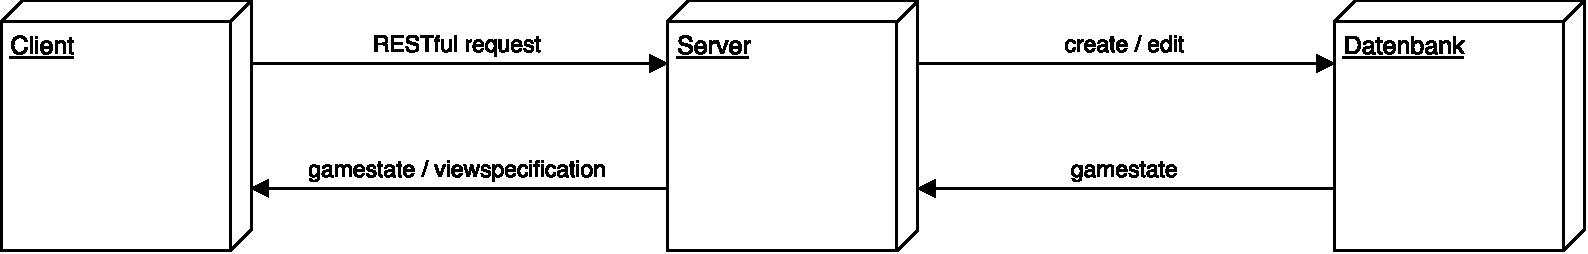
\includegraphics[scale=0.4]{./../Diagrams/Architecture.pdf}
\end{center}
\end{frame}

\section{Objekt Design}
\begin{frame}
\frametitle{Outline}
\begin{enumerate}
\item Mancala
\item Technologien
\item Architektur
\item \textbf{Objekt Design}
\item Demo
\item Frontend
\item Backend
\item Ausblick
\end{enumerate}
\end{frame}

\begin{frame}
\frametitle{Outline}
\begin{enumerate}
\item Mancala
\item Technologien
\item Architektur
\item \textbf{Objekt Design}
\begin{enumerate}
\item Anwendungsfalldiagram
\item Klassendiagram
\item Sequenzdiagram
\end{enumerate}
\item Demo
\item Frontend
\item Backend
\item Ausblick
\end{enumerate}
\end{frame}

\subsection{Use Case Diagram}
\begin{frame}
\frametitle{Outline}
\begin{enumerate}
\item Mancala
\item Technologien
\item Architektur
\item Objekt Design
\begin{enumerate}
\item \textbf{Anwendungsfalldiagramm}
\item Klassendiagramm
\item Sequenzdiagramm
\end{enumerate}
\item Demo
\item Frontend
\item Backend
\item Ausblick
\end{enumerate}
\end{frame}

\begin{frame}
\frametitle{Anwendungsfalldiagramm}
\begin{center}
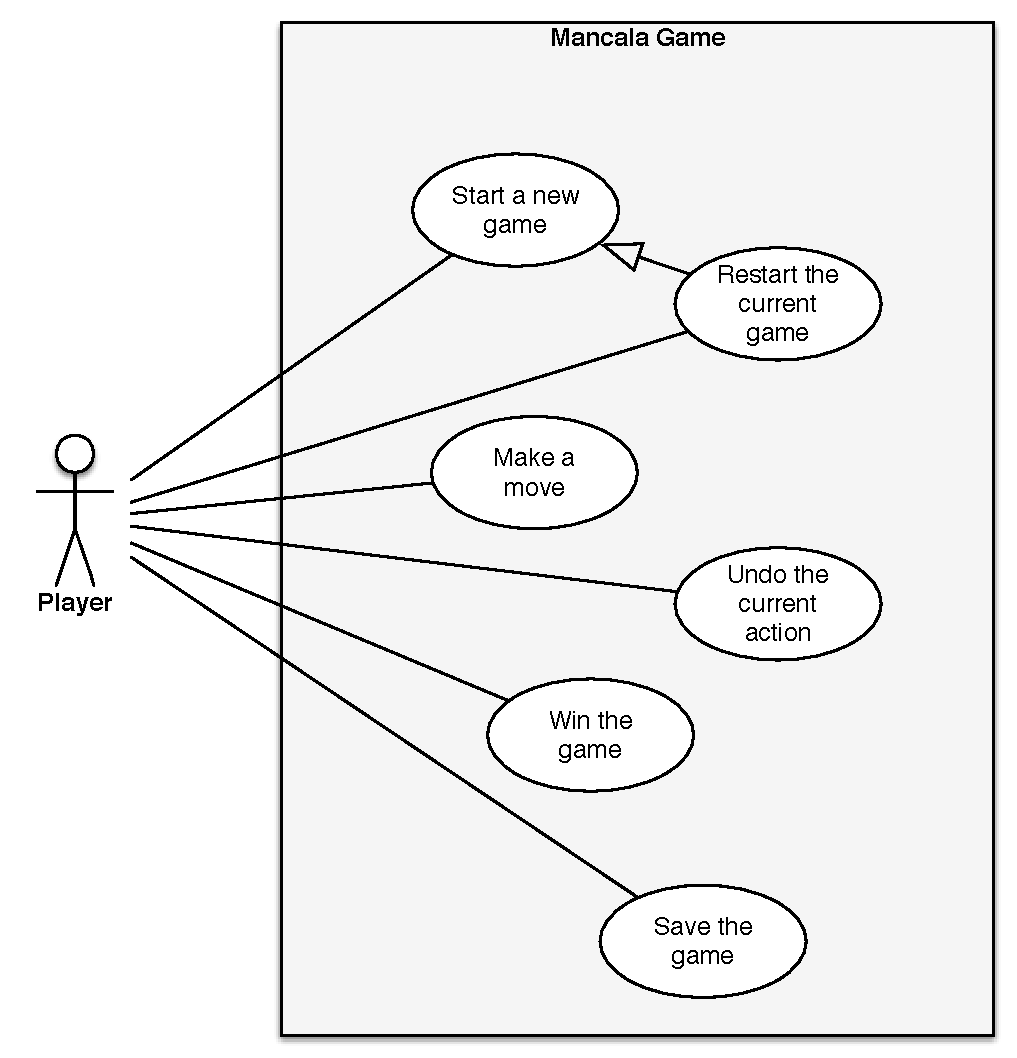
\includegraphics[scale=0.32]{./../Diagrams/UseCases.pdf}
\end{center}
\end{frame}

\subsection{Class Diagram}
\begin{frame}
\frametitle{Outline}
\begin{enumerate}
\item Mancala
\item Technologien
\item Architektur
\item Objekt Design
\begin{enumerate}
\item Anwendungsfalldiagramm
\item \textbf{Klassendiagramm}
\item Sequenzdiagramm
\end{enumerate}
\item Demo
\item Frontend
\item Backend
\item Ausblick
\end{enumerate}
\end{frame}

\begin{frame}
\frametitle{Klassendiagramm}
\begin{center}
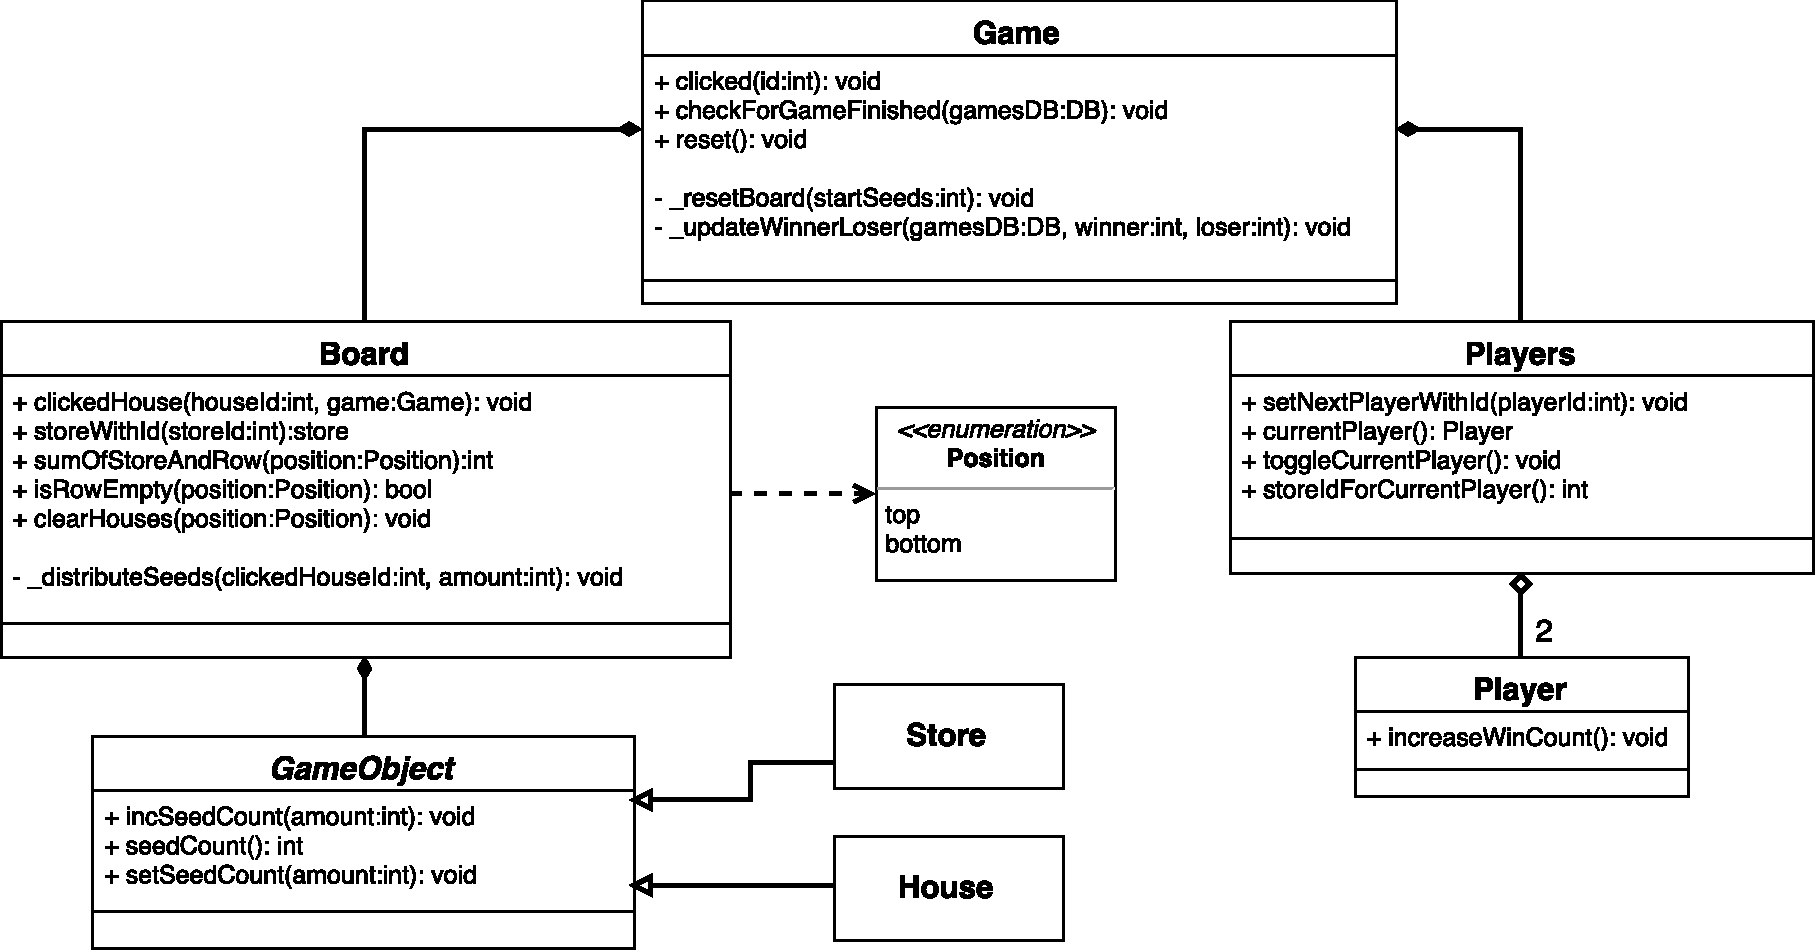
\includegraphics[scale=0.32]{./../Diagrams/Classes.pdf}
\end{center}
\end{frame}

\subsection{Sequenzdiagramm}
\begin{frame}
\frametitle{Outline}
\begin{enumerate}
\item Mancala
\item Technologien
\item Architektur
\item Objekt Design
\begin{enumerate}
\item Anwendungsfalldiagramm
\item Klassendiagram
\item \textbf{Sequenzdiagramm}
\end{enumerate}
\item Demo
\item Frontend
\item Backend
\item Ausblick
\end{enumerate}
\end{frame}

\begin{frame}
\frametitle{Sequenzdiagramm}
\begin{center}
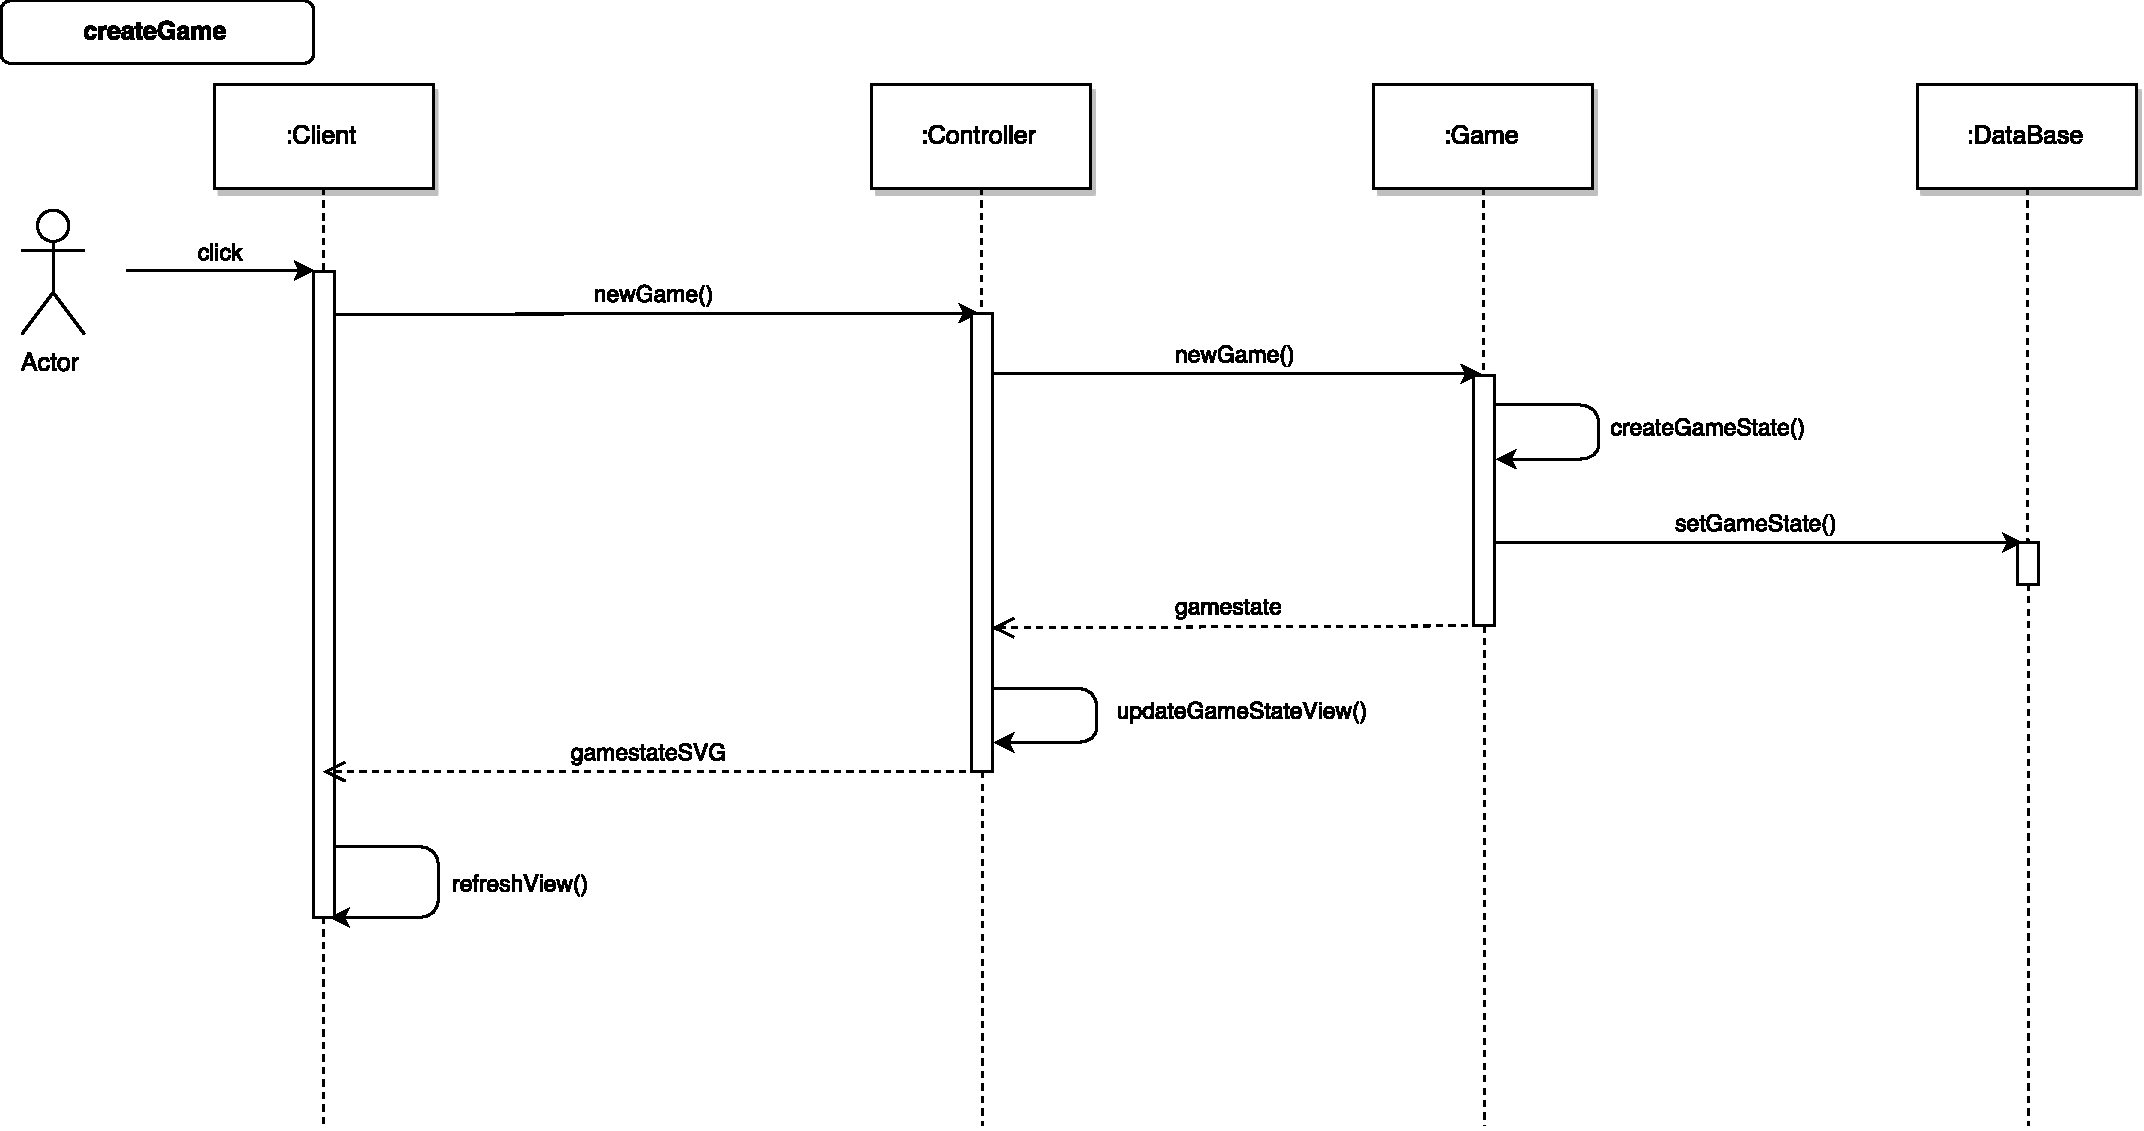
\includegraphics[scale=0.25]{./../Diagrams/Sequence_createGame.pdf}
\end{center}
\end{frame}

\begin{frame}
\frametitle{Sequenzdiagramm}
\begin{center}
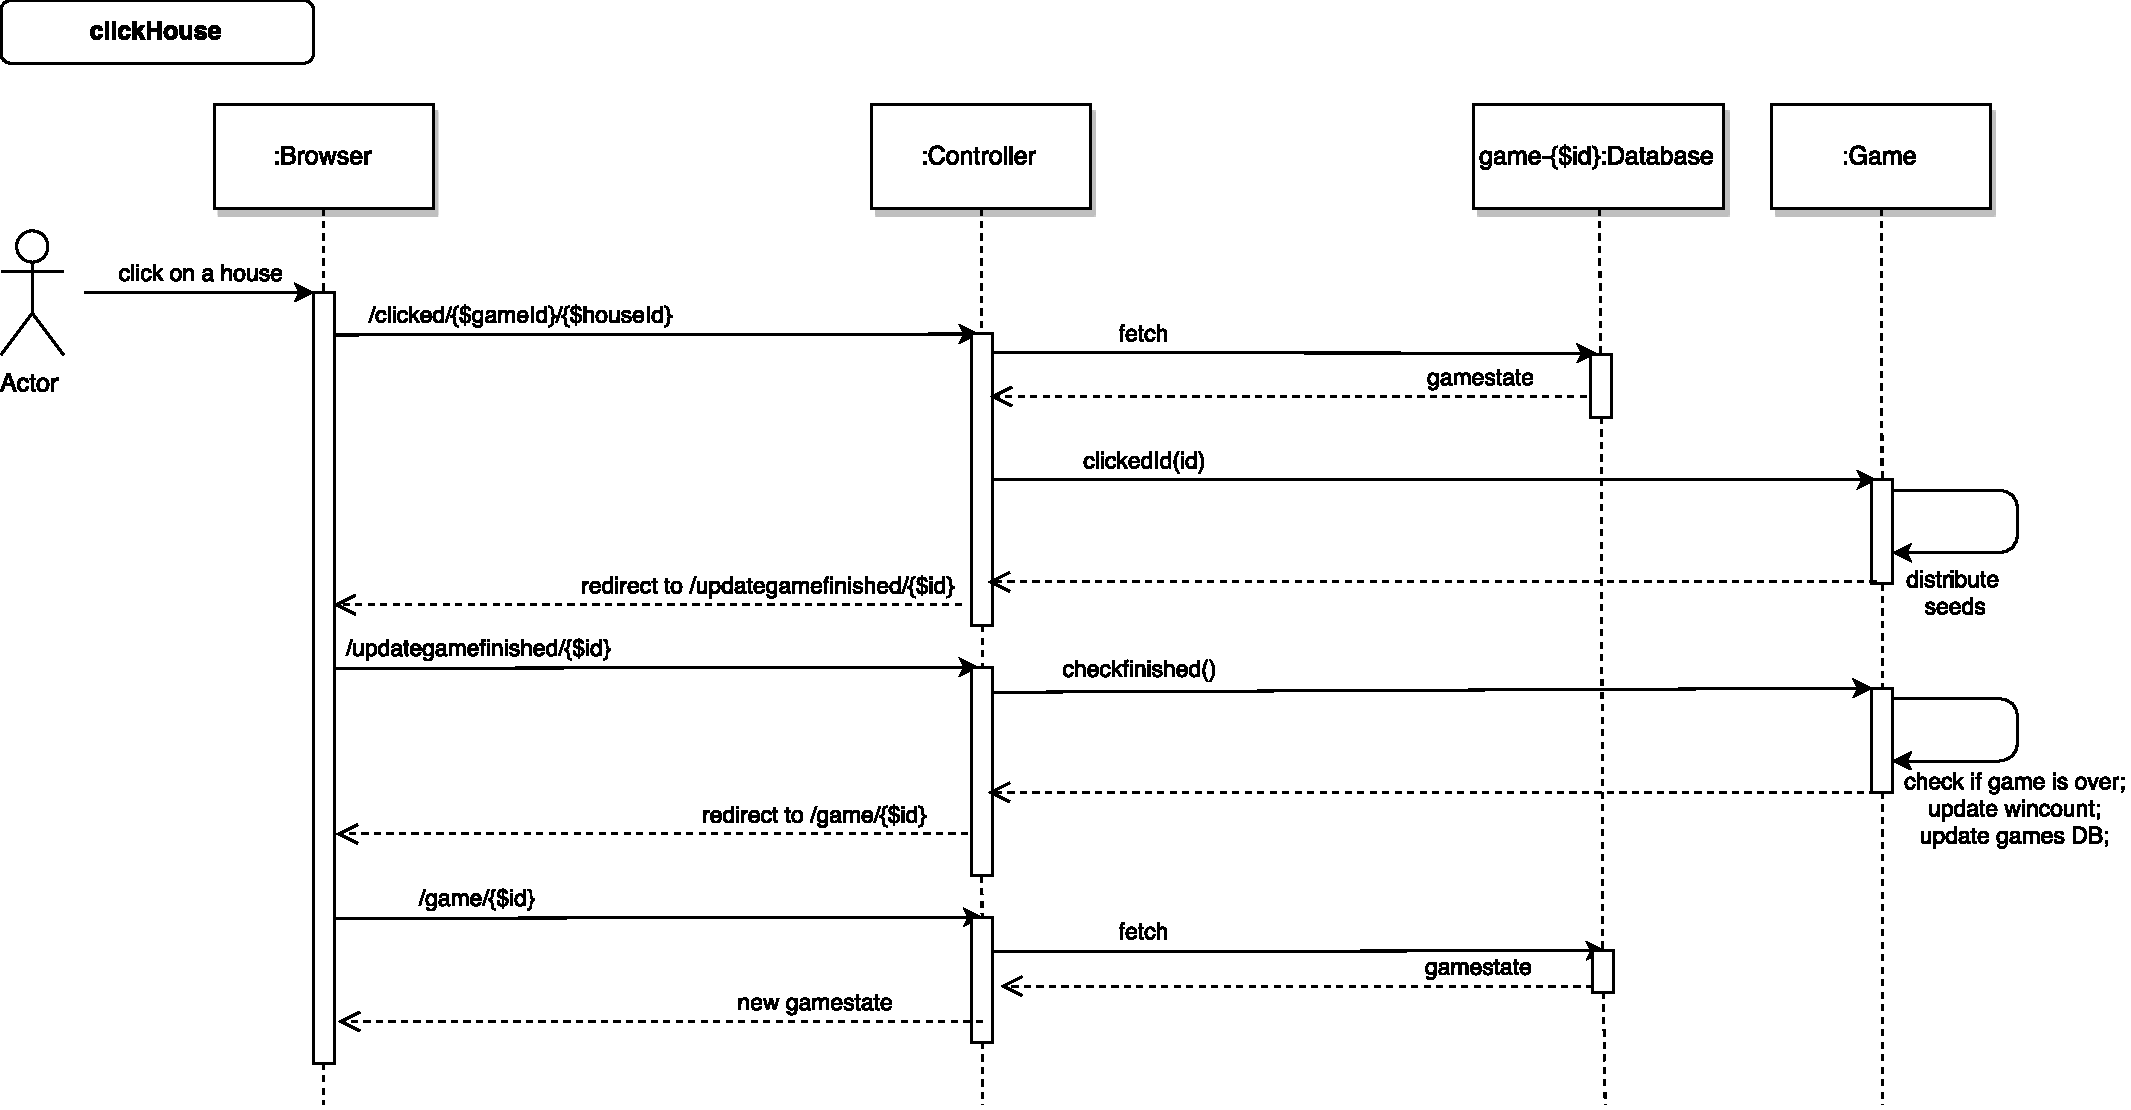
\includegraphics[scale=0.32]{./../Diagrams/Sequence_clickHouse.pdf}
\end{center}
\end{frame}

\section{Demo}
\begin{frame}
\frametitle{Outline}
\begin{enumerate}
\item Mancala
\item Technologien
\item Architektur
\item Objekt Design
\item \textbf{Demo}
\item Frontend
\item Backend
\item Ausblick
\end{enumerate}
\end{frame}

\begin{frame}[plain, c]
\begin{center}
\Large Demo
\end{center}
\end{frame}

\section{Frontend}
\begin{frame}
\frametitle{Outline}
\begin{enumerate}
\item Mancala
\item Technologien
\item Architektur
\item Objekt Design
\item Demo
\item \textbf{Frontend}
\item Backend
\item Ausblick
\end{enumerate}
\end{frame}

\begin{frame}
\frametitle{Frontend}
+\hspace*{-0.8cm}
+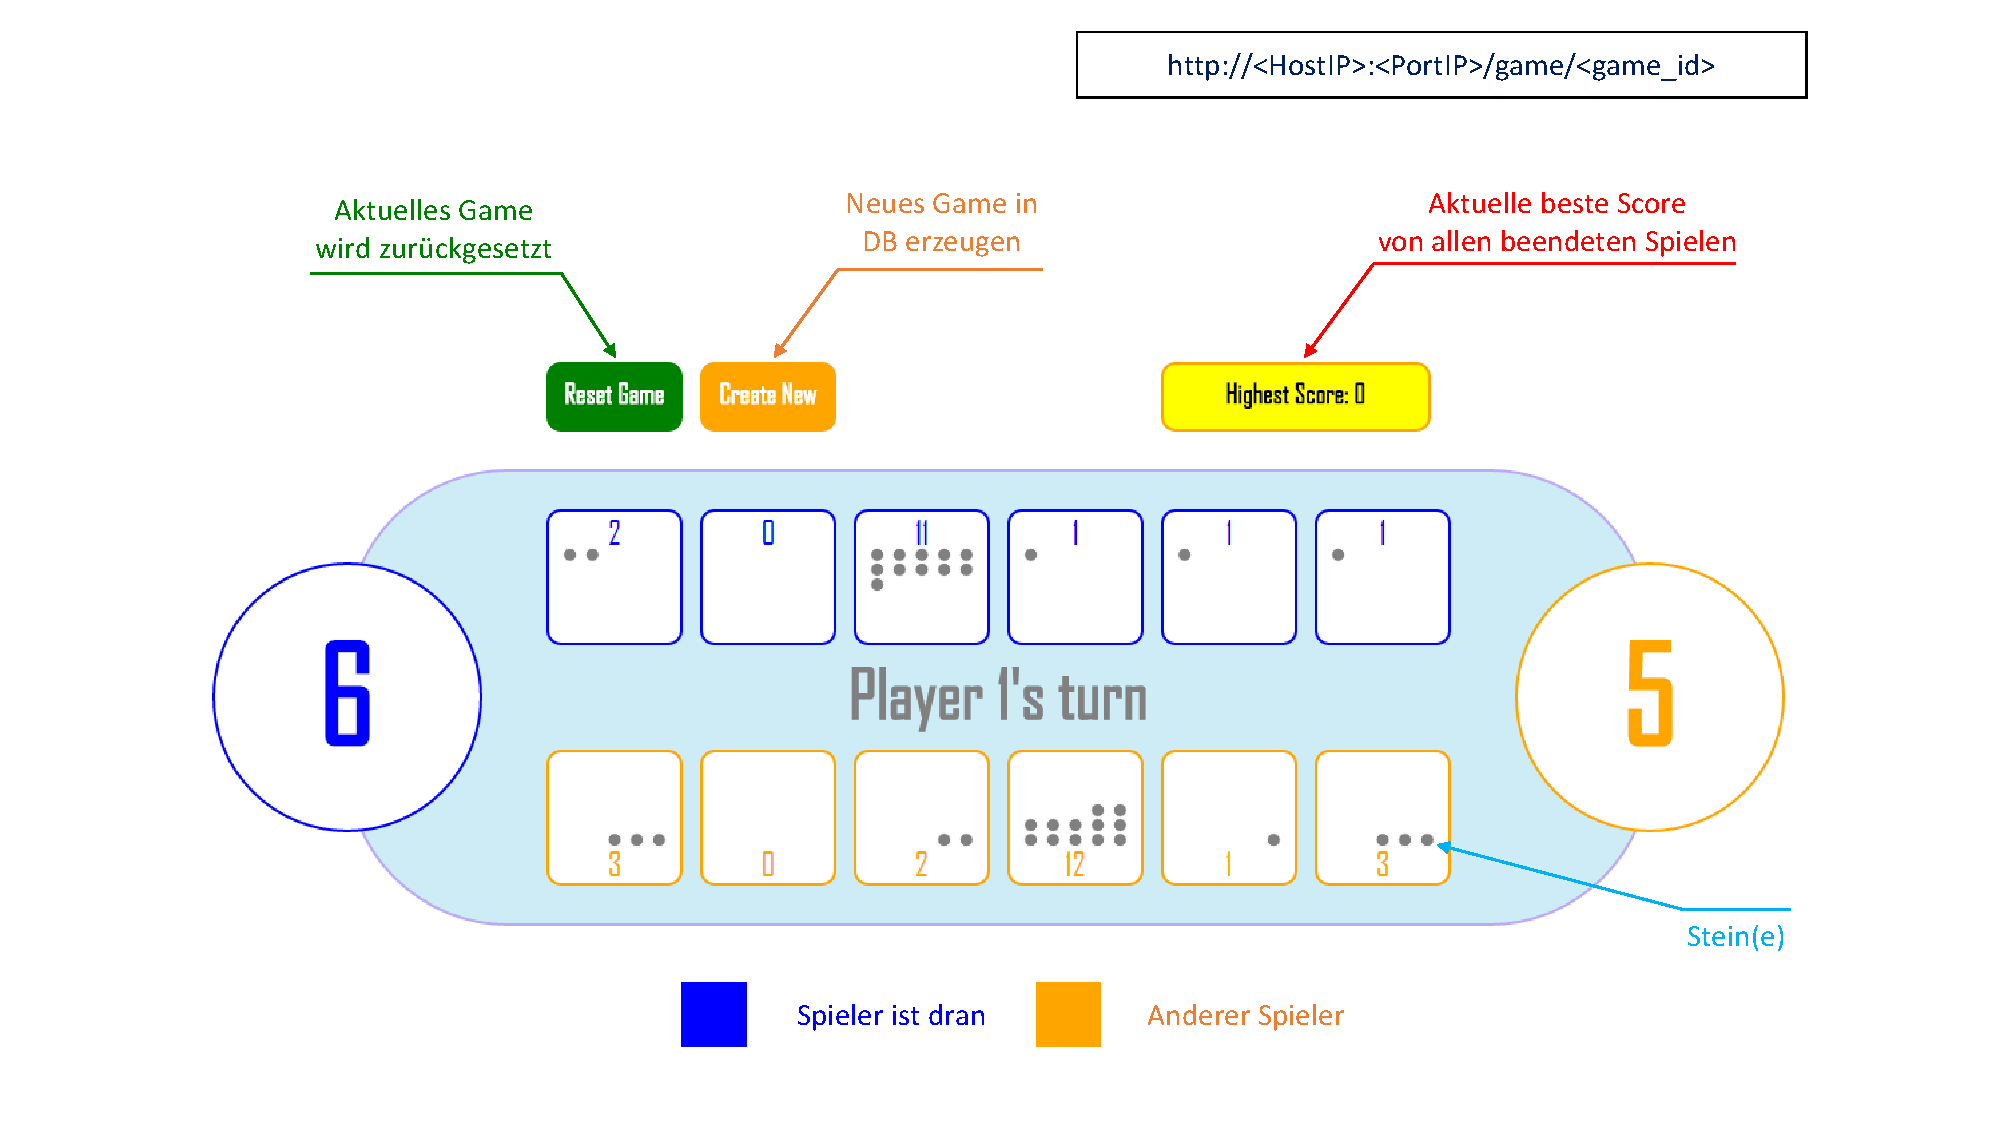
\includegraphics[scale=0.36]{./pictures/GUI_Explanation.pdf}
\end{frame}

\section{Backend}
\begin{frame}
\frametitle{Outline}
\begin{enumerate}
\item Mancala
\item Technologien
\item Architektur
\item Objekt Design
\item Demo
\item Frontend
\item \textbf{Backend}
\item Ausblick
\end{enumerate}
\end{frame}

\begin{frame}
\frametitle{Backend}
\begin{itemize}
\item OOP
\begin{itemize}
\item one xqm per class
\item one namespace per class
\item private methods prefixed with \_
\end{itemize}
\item Databases
\begin{itemize}
\item one index database
\item one database per game
\end{itemize}
\item Problems
\begin{itemize}
\item FLOWR vs update: 
\begin{itemize}
\item Use getter instead of \texttt{let}
\item Use recursion instead of loop
\item Redirect frontend to other url for updated database
\end{itemize}
\item Single node updates:\\
\quad Precompute every value before updating a node
\end{itemize}
\end{itemize}

\end{frame}

\section{Future}
\begin{frame}
\frametitle{Outline}
\begin{enumerate}
\item Mancala
\item Technologien
\item Architektur
\item Objekt Design
\item Demo
\item Frontend
\item Backend
\item \textbf{Ausblick}
\end{enumerate}
\end{frame}

\begin{frame}
\frametitle{Ausblick}
\begin{itemize}
\item ``Klauen'' Regel
\item Distributed Multiplayer
\item KI Gegner
\item User Ranking
\end{itemize}
\end{frame}

\section{Questions}
\begin{frame}[plain, c]
\begin{center}
\Large Vielen Dank!
\end{center}
\end{frame}

\end{document}
